\documentclass{article}
\usepackage[utf8x]{inputenc}
\usepackage[english]{babel}

%Math symbols
\usepackage{amsmath}
\usepackage{amssymb}
\let\oldPr\Pr
\renewcommand{\Pr}[1]{\text{Pr} \left( #1 \right)}
\newcommand{\E}[1]{\mathbb{E} \left[ #1 \right]}
\newcommand{\fancyS}{\mathcal{S}}
\newcommand{\fancyA}{\mathcal{A}}

%Theorems
\newtheorem{definition}{Definition}
\newtheorem{theorem}{Theorem}
\newtheorem{corollary}[theorem]{Corollary}
\newtheorem{lemma}[theorem]{Lemma}
\newtheorem{assumption}{Assumption}

%Figures
\usepackage{graphicx}
\usepackage{float}

%Bibliography
\usepackage{natbib}
\makeatletter
\renewcommand{\@biblabel}[1]{[#1]\hfill}
\makeatother

%Title
\title{MDP Analysis for Blockchain}
\author{Roi Bar Zur \and Ittay Eyal \and Aviv Tamar}
\date{}

\begin{document}

\maketitle

\begin{abstract}
    TODO: Add abstract
\end{abstract}

\section{Introduction}

\subsection{}
TODO: Intro

\subsection{Contributions}
TODO: short paragraph

These are our contributions:
\begin{enumerate}
    \item Designing a novel method to solve Blockchain protocols modeled as MDPs
    \item Proved the new method converges to the optimal solution and bounded the approximation error.
    \item Recreated the approximately optimal results of \cite{sapirshtein2016optimal} for Bitcoin.
    \item Surpassed the results of \cite{hou2019squirrl} for Ethereum.
    \item Analyzed our new method's running time and showed it is more efficient than the current state of the art method (\cite{sapirshtein2016optimal}).
    \item Empirical analysis of the trade-off between running time and approximation error.
\end{enumerate}

TODO: Add navigation paragraph

\section{Related Work}
TODO: Go over related work

Eyal and Sirer were the first to show that the Bitcoin protocol is not incentive compatible (\cite{eyalmajority}). They have demonstrated and analyzed a strategy (called selfish mining or SM1) which can be used by miners and yields higher rewards than acting honestly. Selfish mining involves withholding newly minted blocks and violating the longest chain rule. The existence of such a strategy rules out the honest protocol as a Nash equilibrium.

The analysis in \cite{eyalmajority} gives a closed form formula of the revenue a miner can get if she uses SM1. The formula depends on 2 parameters which model the miner:
\begin{enumerate}
    \item $\alpha \in [0, \frac{1}{2})$ - The miner's relative computational power in respect to the entire network.
    \item $\gamma \in [0, 1]$ - The miner's network connectivity.
\end{enumerate}
The Bitcoin protocol specifies that in the case of a tie in the longest chain rule, the tie is decided in favor of the first chain seen. This is the reason that $\gamma$ is important. In case the selfish miner releases a chain of her own, the more connected she is to other parties in the network, the more parties will favor her chain.

The analysis in \cite{eyalmajority} also finds the threshold for $\alpha$ such that using SM1 is superior to following the protocol. This threshold is a function of $\gamma$. An attacker with a relative power higher than the threshold can use SM1 and obtain more than her fair share. However, the analysis does not guarantee that an attacker with a relative power lower than the threshold cannot deviate in some other way and profit. This means that the SM1 threshold is an upper bound on the security threshold of the protocol. Overall, this analysis implies that under the reasonable assumption of $\gamma = 0.5$ the security threshold of Bitcoin is 0.25 at most.

Sapirshtein et al.~modeled the Bitcoin protocol as an MDP and solved the MDP in order to obtain approximately optimal strategies (\cite{sapirshtein2016optimal}). Their analysis yields an accurate approximation of the security threshold of Bitcoin. For example, they found that for $\gamma = 0.5$, the threshold is as low as 0.231. However, the MDP they obtained is not standard because its objective function is not linear in the reward. In order to overcome this issue they proved that it is possible to approximate the solutions by performing a binary search and solving a standard linear reward MDP in every stage. This method yields a close approximation but is computationally expensive.

Other works have tried to generalize the SM1 strategy to Ethereum and analyze its revenue in order to get an upper bound on the security threshold of Ethereum (\cite{ritz2018impact}, \cite{feng2019selfish}, \cite{grunspan2019selfish}). \cite{ritz2018impact} used a Monte-Carlo simulation in order to assess the revenue of their generalized SM1 strategy while \cite{feng2019selfish} and \cite{grunspan2019selfish} used a theoretical analysis. Nevertheless, all of these works analyze a specific strategy and therefore can only strive to obtain an upper bound of the security threshold.

A recent work by Charlie Hou, Mingxun Zhou and other demonstrates a new technique (which they call SquirRL) to analyze blockchain protocols (\cite{hou2019squirrl}). This method is based on the binary search method of \cite{sapirshtein2016optimal} but instead of solving an MDP in every stage they use Q-Learning.

Briefly, Q-Learning is a method to solve a problem which could be modeled as an MDP but the rewards and transition probabilities are unknown. Q-Learning is somewhat similar to standard MDP solution methods but in addition it learns the rewards and transition probabilities simultaneously. In addition, Q-Learning can work with a large state space by using function approximation, e.g., neural networks.

In \cite{hou2019squirrl}, they choose Q-Learning mostly because of this advantage. Overall, they use SquirRL for Bitcoin and Ethereum and they obtain a better upper bound for the security threshold of Ethereum. By observing their results for bitcoin and comparing to \cite{sapirshtein2016optimal}, they deduce that their method typically finds solutions with revenues approximately 1-2\% lower than the optimum. This leaves room to improve the security threshold of Ethereum.

To our knowledge, no other work has fully solved an MDP of Ethereum. The main obstacle of modeling Ethereum as an MDP explicitly and then solving it is the large number of states which are required since the introduction of uncle rewards complicates the state space.

\section{Name TBD}


TODO: Think of a name for the method (Random stop etc.)
\subsection{Motivation}
TODO: Explain the motivation behind 


\subsection{Markov Decision Process}
TODO: Add short explanation
TODO: Check if necessary for related work

\subsection{Method}
TODO: Go over model description
The main challenge for solving blockchain MDPs is the non-linear reward function. In general the absolute reward of the miner which she wants to maximize is defined as:
\begin{gather*}\label{original_AR_def}
    AR_a = \E{\lim\limits_{T\to\infty} \frac{\sum\limits_{t=1}^T R_t}{\sum\limits_{t=1}^T D_t}}
\end{gather*}
Where $R_t$ is the reward the miner receives in step $t$ and $D_t$ is the contribution of the step $t$ towards the difficulty adjustment. In Bitcoin for example, the difficulty contribution is the sum of rewards all parties receive. Thus $AR_a$ is equivalent to the relative revenue of the miner. In Ethereum, the difficulty contribution in step $t$ is the amount of the amount of blocks added to the main chain and as uncles. This is since in Ethereum uncle blocks are also considered for the difficulty adjustment. This target function is non-linear in the rewards and therefore standard MDP solution methods will not work.

Our method of solving an MDP of this form consists of two stages:
\begin{enumerate}
    \item Constructing an auxiliary MDP (marked by MDP') based on the original MDP. The new MDP' has the same state space as the original MDP and is essentially a duplicate of the original MDP. But MDP' is constructed such that every transition in it has some chance to end the process and move to a finite state. If this does not happen then the transition occurs as in the original MDP.
    At every transition, the chance to end abruptly is $(1 - \frac{1}{D})^{D_t}$ where $D$ is some chosen parameter.\\
    The objective function of MDP' is:
    \begin{gather*}
        R = \E{\frac{1}{D} \sum\limits_{t=0}^\text{Term} R_t}
    \end{gather*}
    where Term is a random variable indicating the step in which the process terminates. This is essentially a discounted reward with $\beta = 1$ and setting $R_t = 0$ for all $t > \text{Term}$.
    \item Solving MDP' using standard MDP solver algorithms (i.e. Value Iteration) to obtain an approximately optimal policy.
\end{enumerate}

Note that the chance to end the process abruptly depends on $D_t$ and the higher $D_t$ is, the higher the chance to end the process. Intuitively, this encourages consideration of how actions add to the difficulty contribution and finding a balance between the reward added and the difficulty contribution. We call $D$ the expected horizon since this is the expected total difficulty contribution when the process ends (this will be explained formally in the theoretical results section).

Then, in order to analyze the revenue of the policy we find the steady-state probability of the Markov chain induced by applying the policy our method finds to the original MDP. We then use the steady-state probability distribution to calculate the expected reward and expected difficulty contribution of each step. The absolute revenue is then the ratio between the two values.

An important thing to notice is that our method involves solving a single MDP only. Therefore, it should be considerably more efficient than the binary search of \cite{sapirshtein2016optimal}. However, there should be a trade-off between the running time and the approximation error of the result and one of our goals is to characterize this trade-off.

An enhancement of our method that seems to work even better is creating a new MDP which consists of $k$ sections where each section is similar to MDP' and instead of giving every transition a chance to end the process, we give every transition in the first $k - 1$ sections a chance to move to the next section. Only in the last section, we give each transition a chance to end the process. This is basically $k$ MDP's played one after another. This method seems to work better but needs to be researched further to formally understand its properties.

\subsection{Proof of Optimality}
TODO: Add overview of theorems for equivalence

\subsection{Approximation Error}
TODO: Add overview of theorems for bounding the error

\section{Results}

\subsection{Optimality results}
\subsubsection{Bitcoin}
TODO: go over results
Recreated \cite{sapirshtein2016optimal}:
\begin{center}
\begin{tabular}{ |c|c|c|c| } 
 \hline
 Power ($\alpha$) & Connectivity ($\gamma$) & Revenue ($AR_a$) & Revenue in \cite{sapirshtein2016optimal}\\
 \hline
 0.35 & 0 & 0.370773 & 0.37077\\
 \hline
 0.4 & 0 & 0.488634 & 0.48863\\
 \hline
 0.45 & 0 & 0.668149 & 0.66809\\
 \hline
\end{tabular}
\end{center}

In comparison to \cite{hou2019squirrl}, their method obtains results about 1\% lower than \cite{sapirshtein2016optimal} and our method easily surpasses theirs.

\subsubsection{Ethereum}
After building a model for an MDP which represents the Ethereum blockchain and using our method we managed to get new results:
\begin{center}
\begin{tabular}{ |c|c| } 
 \hline
 Power ($\alpha$) & Revenue ($AR_a$)\\
 \hline
 0.2469 & 0.246912\\
 \hline
 0.247 & 0.247033\\
 \hline
 0.25 & 0.250705\\
 \hline
 0.3 & 0.317798\\
 \hline
 0.35 & 0.407925\\
 \hline
 0.4 & 0.534359\\
 \hline
\end{tabular}
\end{center}
Notice that the new threshold we found is 0.2469. This is lower than state of the art results which are approximately 0.26 (\cite{ritz2018impact}, \cite{feng2019selfish}).

\subsection{Running Time Comparison}
TODO: Compare method performance for a limited running time Sapirshtein vs. ours

\section{Hyperparameters}

\subsection{Expected Horizon}
TODO: Go over this, Graph for expected horizon
Although it is yet unproven that our method converges to the optimal solution, the fact that it outshines other methods and the preliminary analysis we have performed lead us to believe that it does converge to the optimum. Figure \ref{fig:empirical_results} shows the revenue of the resulting policy our method finds against the horizon length considered. As the considered horizon increases the revenue seems to converge to some optimum.
\begin{figure}[H]
    \centering
    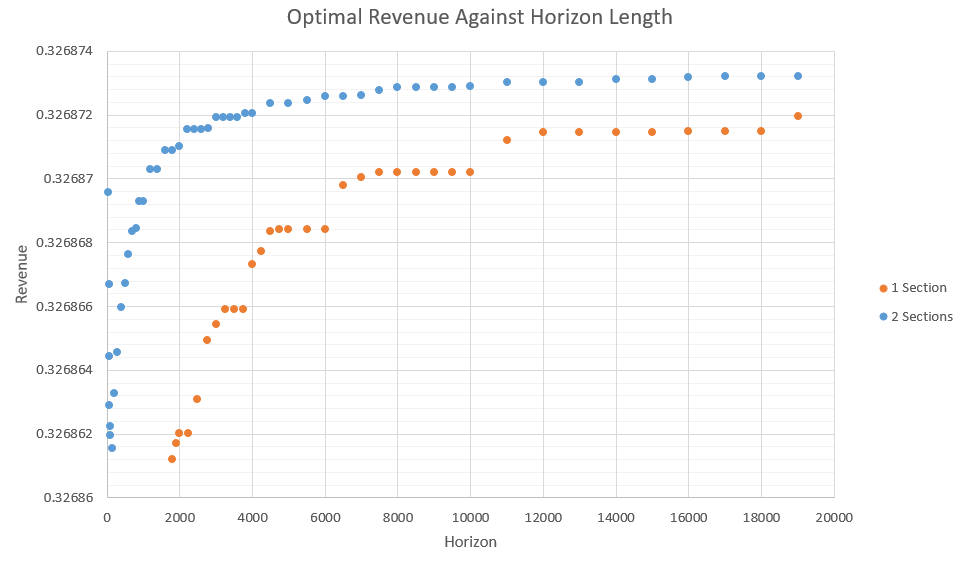
\includegraphics[width=\textwidth]{graph1.png}
    \caption{Our method's results for Bitcoin with a $\alpha = 0.3, \gamma = 0.5$ and limiting the maximum fork length to 20}
    \label{fig:empirical_results}
\end{figure}

\subsection{Maximal Fork Length}
TODO: Graph for max fork
Show that this is negligible for fork > 20


\section{Proofs}
TODO: Go over this and add from other doc
TODO: Move to addendum?

\subsection{Original MDP}
\begin{definition}
    The absolute revenue of the attacker in the original MDP is:
    \begin{gather*}
        \text{AR}_1 \triangleq \E{\lim\limits_{T\to\infty} \frac{\sum\limits_{t=1}^T R_t}{\sum\limits_{t=1}^T D_t}}
    \end{gather*}
\end{definition}
We make the easing assumption that at every step the maximal contribution to the difficulty is upper bounded by some constant $c$. Formally:
\begin{assumption}
    $\forall_t : 0 \leq D_t \leq c$
\end{assumption}

\subsection{Intermediary MDP}
We define an intermediary MDP which will serve to prove that optimizing the original MDP is the same as optimizing the linear reward MDP we construct in our method. The intermediary MDP is finite and stops exactly when the difficulty contribution passes the chosen parameter $D$.
\begin{definition}
    The step in which the intermediary MDP terminates is defined as:
    \begin{gather*}
        \text{Term}_2(D) \triangleq \arg \min\limits_T \{ \sum\limits_{t=1}^T D_t \geq D \}
    \end{gather*}
\end{definition}
\begin{definition}
    The absolute revenue of the attacker in the intermediary MDP is:
    \begin{gather*}
         \text{AR}_2 \triangleq \E{\lim\limits_{D\to\infty} \frac{\sum\limits_{t=1}^{\text{Term}_2(D)} R_t}{\sum\limits_{t=1}^{\text{Term}_2(D)} D_t}}
    \end{gather*}
\end{definition}
\begin{lemma}\label{inter_orig_ar_eq}
    The absolute revenue of the original MDP is equivalent to the absolute revenue of the intermediary MDP.
    \begin{gather*}
        \text{AR}_1 = \text{AR}_2
    \end{gather*}
\end{lemma}
We have already proved this lemma but will leave the proof out of the proposal.

\subsection{Linear Reward MDP}
The MDP we construct using our method has a linear reward function and thus can be solved using standard MDP solution methods. We would like to show that optimizing this MDP is the same as optimizing the original MDP and will do so by comparing this MDP to the intermediary MDP.
\begin{definition}
    At every step $t$, $X_t$ is a random variable indicating whether the process terminated 0at this step. It is defined as:
    \begin{gather*}
        X_t \triangleq
        \begin{cases}
            1 & \text{w.p } \left( 1 -\frac{1}{D} \right)^{D_t} \text{ (continue)} \\
            0 & \text{w.p } 1 - \left( 1 -\frac{1}{D} \right)^{D_t} \text{ (stop)} \\
            \end{cases}
    \end{gather*}
\end{definition}
\begin{definition}
    The step in which the linear reward MDP terminates is defined as:
    \begin{gather*}
        \text{Term}_3(D) \triangleq \arg \min\limits_T \{ X_T = 0 \}
    \end{gather*}
\end{definition}
\begin{definition}
    The absolute revenue of the attacker in the linear reward MDP we defined is:
    \begin{gather*}
         \text{AR}_3 \triangleq \E{\lim\limits_{D\to\infty} \frac{1}{D}\sum\limits_{t=1}^{\text{Term}_3(D)} R_t}
    \end{gather*}
\end{definition}
A handy lemma which we have already proved:
\begin{lemma}
    The expected total contribution to the difficulty when the linear reward MDP terminates is asymptotically equivalent to $D$. Formally:
    \begin{gather*}
        \E{\lim\limits_{D\to\infty} \frac{1}{D} \sum\limits_{t=1}^{\text{Term}_3(D)} D_t} = 1
    \end{gather*}
\end{lemma}
This lemma is the reason we call $D$ the expected horizon. Intuitively, For a large enough $D$, the expected sum of the difficulty contribution from the start of the process until termination is close to $D$.

In order to show that optimizing the linear reward MDP is equivalent to optimizing the intermediary MDP we will prove the following theorem:
\begin{theorem}\label{lin_inter_ar_eq}
    The absolute revenue of the intermediary MDP is equivalent to the absolute revenue of the linear reward MDP.
    \begin{gather*}
        \text{AR}_2 = \text{AR}_3
    \end{gather*}
\end{theorem}
Assuming theorem \ref{lin_inter_ar_eq} is true, thanks to lemma \ref{inter_orig_ar_eq}, we immediately get:
\begin{corollary}
    Optimizing the original MDP is the same as optimizing the linear reward MDP constructed by our method.
    \begin{gather*}
        \text{AR}_1 = \text{AR}_3
    \end{gather*}
\end{corollary}
And this would conclude the proof that our method converges the optimal solution.

\section{Discussion and Future Work}
TODO: Add

\section{Conclusion}
TODO: Add

\bibliographystyle{alpha}
\bibliography{refs}

\end{document}
